%\documentclass[12pt, a4paper]{article}
\documentclass[prb,preprint]{revtex4} 


\usepackage{amsmath}
\usepackage{amsfonts}
\usepackage{amssymb}
\usepackage{physics}
\usepackage{mathtools}
\usepackage{verbatim}


\usepackage{graphicx}

\usepackage[amsthm, framed]{ntheorem}

\usepackage[colorlinks,citecolor=blue,urlcolor=blue,bookmarks=false,hypertexnames=true]{hyperref} 
%\usepackage{amsmath}
\DeclareMathOperator*{\argmax}{arg\,max}
\DeclareMathOperator*{\argmin}{arg\,min}

%\usepackage{mathtools}
\DeclarePairedDelimiter\ceil{\lceil}{\rceil}
\DeclarePairedDelimiter\floor{\lfloor}{\rfloor}
%\DeclarePairedDelimiter{\abs}{\lvert}{\rvert}

%\usepackage[amsthm, framed]{ntheorem}
\newtheorem{theorem}{Theorem}
\newtheorem{definition}{Definition}
\newtheorem{proposition}{Proposition}
\newtheorem{insight}{Insight}
\newtheorem*{problem*}{Problem}

% Complexity theory
\newcommand\bigO[1]{\mathcal{O}(#1)}

\begin{document}
	

\title{Explaining quantum phase estimation using data structures}
\date{\today}
\begin{abstract}
	The quantum phase estimation algorithm is an fundamental technique for performing physical simulation tasks on quantum computers. 
	Most existing presentations of quantum phase estimation proceed by first stating the quantum circuit for phase estimation and then using an algebraic manipulation to prove its correctness. Such a presentation can be unsatisfactory as it does not explain quantum phase estimation by appeal to any algorithmic ideas.
	This paper explains the phase estimation algorithm in a new way, using elementary polynomial data structures from computer science as helpful high-level concepts. 
	Once the polynomial data structure concepts have been understood, the explanation of quantum phase estimation can be stated in just a few lines.
	We hope this alternative approach to explaining phase estimation will help instructors as quantum computing grows in popularity and is taught in more diverse contexts.
\end{abstract}
\maketitle



%\author{Shashvat Shukla}

\section{Introduction}

% What are the goals of the introduction? 
% Demonstrate usefulness, interestingness, accessibility, novelty and broad appeal
% also: connection to data structures and algorithms

%A paper's introductory section must provide the background and context that a typical physicist, regardless of area of specialization, would need in order to understand the paper's purpose and importance. That is, it should motivate the paper, in a way that is both informative and inviting. Unlike the abstract, the introduction need not summarize the entire paper or state its main results. Often, however, the introduction ends with a paragraph that outlines how the rest of the paper is organized; this is especially useful for longer papers.
	
% quantum computing, quantum algorithms, quantum phase estimation
Quantum computers promise new algorithms for solving problems that are intractable on classical computers \cite{nielsen2010quantum}. Their power comes from quantum bits (qubits), which, unlike classical bits, can exploit superposition, interference, and entanglement to store and process information more efficiently. Among the most important algorithms that harness this power is quantum phase estimation\cite{kitaev1995quantum}. It is a subroutine in algorithms for the simulation of physical systems\cite{abrams1999quantum} and in Shor’s factoring algorithm\cite{shor1994algorithms}.

% the problem we solve, how we solve it. accessibility, interestingness and connection to other fields. 
Most existing presentations of phase estimation use detailed algebraic derivations\cite{nielsen2010quantum, wong2022introduction}. They generally present the quantum circuit for the algorithm and present an analysis of the correctness of the algorithm by means of algebraic manipulation. While rigorous, they often obscure the underlying ideas and can be tedious especially for settings where a quick, high-level explanation would be sufficient. The usefulness of this paper is in providing an alternative explanation for quantum phase estimation. We show how elementary data structures for representing and multiplying polynomials efficiently and a divide-and-conquer approach can help explain the quantum phase estimation algorithm at a high level. Instructors can consider whether the usual algebraic details are required in their course, and they may opt to leave them to students in the form of homework exercises to be done only after the students are comfortable with the main algorithmic idea.

% why it has broad appeal
An ever-larger community of scientists will need at least a working understanding of phase estimation because quantum computing is a growing scientific area and industry in its own right, and it is expected that it will be applied in various branches of science. With the rapid growth of university courses and programs in quantum computing, many instructors across physics will find themselves teaching or applying it. We hope our conceptual explanation will be helpful to these instructors.
	
\section{Data structures for phase estimation}

This section introduces the concepts that feature in our explanation of quantum phase estimation. We first review classical data structures for representing polynomials, then show how these motivate the Discrete and Fast Fourier transforms, and finally explain the quantum analogues of these ideas. Table~\ref{tbl:data_structures} condenses these concepts and how they are related. 
	

	\subsection{Polynomial data structures}	
	
	% Coefficient representation
	The material in this section can be motivated by asking students to consider how polynomials might be represented in a classical computer. 
	The straightforward approach, the \textbf{coefficient representation} of a polynomial \cite{cormen2009algorithms_ch30} involves storing a vector (or list) of all its coefficients. For example the polynomial $p(x) = a_{N-1}x^{N-1} + ... + a_0$ is stored as the vector $a = [a_0 ... a_{N-1}]$. 
	
	% Point value representation
	There are other data structures for polynomials \cite{cormen2009algorithms_ch30}. Consider the \textbf{point-value representation} of a polynomial \cite{cormen2009algorithms_ch30}, which uses the fact that a polynomial, $p$, with degree less than $N$ is uniquely determined by a set of $N$ distinct points $\{(x_0,p(x_0)), ..., (x_{N-1},p(x_{N-1}))\}$. For example, if we store two points, we represent the unique line that passes through those points. If we fix the inputs $\{x_0, ..., x_{N-1}\}$ at which we will evaluate every polynomial, then we can represent the any polynomial of degree up to $N$ by only storing the values $[p(x_0)...p(x_{N-1})]$ as a vector. We are free to choose any set of $N$ distinct input values for this purpose.
	
	% The coefficient representation makes multiplication easier, dont need to bring in Horner's rule at all
	The point-value representation is significant in classical algorithms because multiplying two polynomials that are represented in this way is efficient. For two polynomials $p$ and $q$, their product $r = p \cdot q$ can be obtained simply by multiplying their stored values coordinate by coordinate:
	\begin{equation}
	[r(x_0), \ldots, r(x_{N-1})] = [p(x_0)q(x_0), \ldots, p(x_{N-1})q(x_{N-1})].
	\end{equation}
	One requirement for this multiplication procedure is that polynomials $p$ and $q$ each have degree less than $N/2$ so that the resulting product $r$ still has degree less than $N$ and can be uniquely determined by $N$ evaluation points. Multiplication of polynomials in the point-value representation only requires $\mathcal{O}(N)$ multiplications of numbers. In contrast, multiplication of polynomials in the coefficient representation requires combining and summing cross-terms, which requires $O(N^2)$ additions and multiplications of numbers.
	
% Switching data structure representations to benefit from the faster multiplication operation
We now motivate the discrete Fourier transform from this perspective. The coefficient representation is the more common and natural choice, so one would hope to store their polynomials in the coefficient representation but use a method to convert between the two representations efficiently in order to take advantage of the faster multiplication algorithm in the point-value representation. The naive approach to converting from coefficients to point values requires multiplying by a Vandermonde matrix. For example, given $p(x) = a_0 + a_1 x + \cdots + a_{N-1}x^{N-1}$ and fixed evaluation points $\{x_0, \ldots, x_{N-1}\}$, the point value representation is obtained by:
\begin{equation}
\begin{bmatrix}
	p(x_0) \\
	p(x_1) \\
	\vdots \\
	p(x_{N-1})
\end{bmatrix}
=
\begin{bmatrix}
	1 & x_0 & x_0^2 & \cdots & x_0^{N-1} \\
	1 & x_1 & x_1^2 & \cdots & x_1^{N-1} \\
	\vdots & \vdots & \vdots & \ddots & \vdots \\
	1 & x_{N-1} & x_{N-1}^2 & \cdots & x_{N-1}^{N-1}
\end{bmatrix}
\begin{bmatrix}
	a_0 \\ a_1 \\ \vdots \\ a_{N-1}
\end{bmatrix}.
\end{equation}

In general multiplying a matrix onto a vector requires $O(N^2)$ elementary operations. Thus we cannot hope to benefit from the $O(N)$ multiplication of the point-value representation if we convert representations in the naive way.
%%%% State how good FFT is and make the link back here so rest of the explanation can just be about FFT

% DFT and FFT
However it is possible to convert representations in $O(N\log N)$ time if we choose the a special set of evaluation points. Specifically, if we choose the $N$-th roots of unity (i.e. powers of $\omega_N = e^{i\frac{2\pi}{N}}$) then the Vandermonde matrix becomes
\begin{equation}
F_N =
\begin{bmatrix}
	1 & 1 & 1 & \cdots & 1 \\
	1 & \omega_N & \omega_N^2 & \cdots & \omega_N^{N-1} \\
	1 & \omega_N^2 & \omega_N^{2\cdot 2} & \cdots & \omega_N^{2(N-1)} \\
	\vdots & \vdots & \vdots & \ddots & \vdots \\
	1 & \omega_N^{N-1} & \omega_N^{2(N-1)} & \cdots & \omega_N^{(N-1)(N-1)}
\end{bmatrix}.
\end{equation}
This matrix $F_N$ is called the discrete Fourier transform (DFT) matrix. Applying it to the coefficient vector $[a_0, \ldots, a_{N-1}]$ computes the values $p(1), p(\omega_N), \ldots, p(\omega_N^{N-1})$. 

The Fast Fourier Transform (FFT) is a divide-and-conquer method to multiply $F_N$ to a vector in only $O(N\log N)$ time, making the conversion between coefficient and point-value representations efficient.

	% Explain the divide and conquer strategy of QFT
	The key idea is to split the $N$ coefficients $(a_0, \ldots, a_{N-1})$ into their even- and odd-indexed parts, forming two smaller polynomials of size $N/2$. These smaller polynomials can be evaluated at all the points more efficiently because some values repeat, and only half as many polynomial evaluations are needed. For instance, since
	\[
	\omega_N^{2(i + N/2)} = \omega_N^{2i}\,\omega_N^{N} = \omega_N^{2i},
	\]
	we have
	\[
	p_{\text{even}}(\omega_N^{i + N/2}) = p_{\text{even}}(\omega_N^i),
	\]
	i.e. the evaluations at $\omega_N^i$ and $\omega_N^{i+N/2}$ are identical for all $i$. This is also true for the odd-indexed part. Then combining the results using simple additions and multiplications by powers of $\omega_N$:
	\begin{equation}
		p(\omega_N^k) = p_{\text{even}}(\omega_N^{2k}) + \omega_N^k\, p_{\text{odd}}(\omega_N^{2k}), \qquad k = 0, \ldots, N/2 - 1.
	\end{equation}
	Recursively applying this decomposition halves the problem size at each step, reducing the total work from $O(N^2)$ to $O(N\log N)$.
		
	
	%%%% Add a figure to illustrate the options of multiplying directly or after conversion
	
	\subsection{Quantum data structures}
	
	% How to motivate this material
	After students have been introduced to the background concepts in the previous section, the material in this section can be motivated as the natural quantum analogues of the concepts in the previous section. 
	
	% Amplitude encoding, ~ of polynomial data structures
	Quantum computers are capable of performing some computations on large vectors efficiently by encoding the data into the amplitudes of a quantum state. Since an $n$ qubit quantum state is described using a vector of $2^n$ amplitudes, computations that encode vectors as quantum states and use them are capable of achieving large advantages in space and time complexity. The standard encoding, known as the \textbf{amplitude encoding} of a vector, is the quantum state obtained by normalising the components of a vector and putting them into amplitudes of a quantum state, for example as: $v= [v_0 ... v_{N-1}] \rightarrow \frac{1}{\norm{v}} \sum_{i=0}^{N-1} v_i \ket{i}$. Our explanation of QPE will feature the \textit{amplitude encodings} of the coefficient and point-value representations of polynomials.%monomials of the form $x^k$. 
	
	% DFT , QFT
	The primary way that quantum computers manipulate these amplitude encoded vectors is by the multiplication of unitary matrices. 
	When normalised by a $\frac{1}{\sqrt{N}}$ factor, the Discrete Fourier Transform is a unitary matrix. If we implement this matrix as a quantum circuit, it converts from the \textit{amplitude encoding} of the coefficient representation to the \textit{amplitude encoding} of the point-value representation. This circuit is called the Quantum Fourier Transform and it can be implemented efficiently due to a divide-and-conquer algorithm which follows a similar logic to the divide-and-conquer approach of the Fast Fourier Transform \cite{paradisi2004presentation}.


\begin{table}[h!]
	\centering
	\renewcommand{\arraystretch}{1.4} % adds vertical space between rows
	\begin{tabular}{|c|c|c|}
		\hline
		\textbf{} & \textbf{Coefficient Representation} & \textbf{Point-value Representation} \\
		\hline
		Classical &
		$[\,a_0 \quad a_1 \quad \dots \quad a_{N-1}\,]$ &
		$[\,p(1) \quad p(\omega_N) \quad \dots \quad p(\omega_N^{N-1})\,]$ \\[1em]
		\hline
		Quantum (Amplitude encoding) &
		$\displaystyle \frac{1}{\|a\|} \sum_{j=0}^{N-1} a_j \, |j\rangle$ &
		$\displaystyle \frac{1}{\sqrt{N}\|a\|} \sum_{j=0}^{N-1} p(\omega_N^j) \, |j\rangle$ \\
		\hline
	\end{tabular}
	\caption{Data structures for storing polynomial $p(x) = a_0 + ... + a_{N-1} x^{N-1}$. The two classical data structures are a list of values or a vector. The two quantum data structures are the amplitude encodings of the same vectors. We can convert from the coefficient representation to the point-value representation by applying the Discrete Fourier Transform in the classical case, and the Quantum Fourier Transform in the quantum case. }
	\label{tbl:data_structures}
\end{table}




	
	\section{Quantum Phase Estimation}
	\label{sec:qpe}
	% Problem and set up
	
	\subsection{Problem}
	We now apply the above concepts to explain quantum phase estimation (QPE). The QPE problem formalizes the task of extracting an eigenvalue of a unitary operator given an eigenstate. 
	%%%% Edit from here. Merge bits of precision thing earlier.
	\begin{problem*}
		Let $U$ denote a unitary matrix, and let $\ket{\psi} \in \mathbb{P}(\mathbb{C}^N)$ be an eigenvector of $U$ with corresponding eigenvalue $\omega_N^k = e^{i 2 \pi k/N}$, where $k\in \mathbb{Z}$ is an unknown.  
		
		Given: 
		\begin{enumerate}
			\item $\ket{\psi}$ as one copy of the quantum state, and
			\item access to $U$ via black-box calls to a qudit-controlled-$U^d$ gate,
		\end{enumerate} 
		the objective is to determine $k$. 
	\end{problem*}
	We define the qudit-controlled-$U^d$ gate, as the gate that acts in the following manner:
	$(C_dU^d) \ket{j}\ket{\phi} = \ket{j}U^j\ket{\phi}$. This is a generalisation of the standard controlled-$U$ gate, which either applies the $U$ gate 0 or 1 times, depending on the controlling register. The qudit-controlled-$U^d$ gate applies the $U$ gate $j$ times, if the number in the controlling register is $j$. This allows us to apply $U$ different numbers of times in a controlled way. 
	
	\subsection{Algorithm}
	
	\begin{figure}
		\centering
		\title{Quantum Phase Estimation Algorithm}
		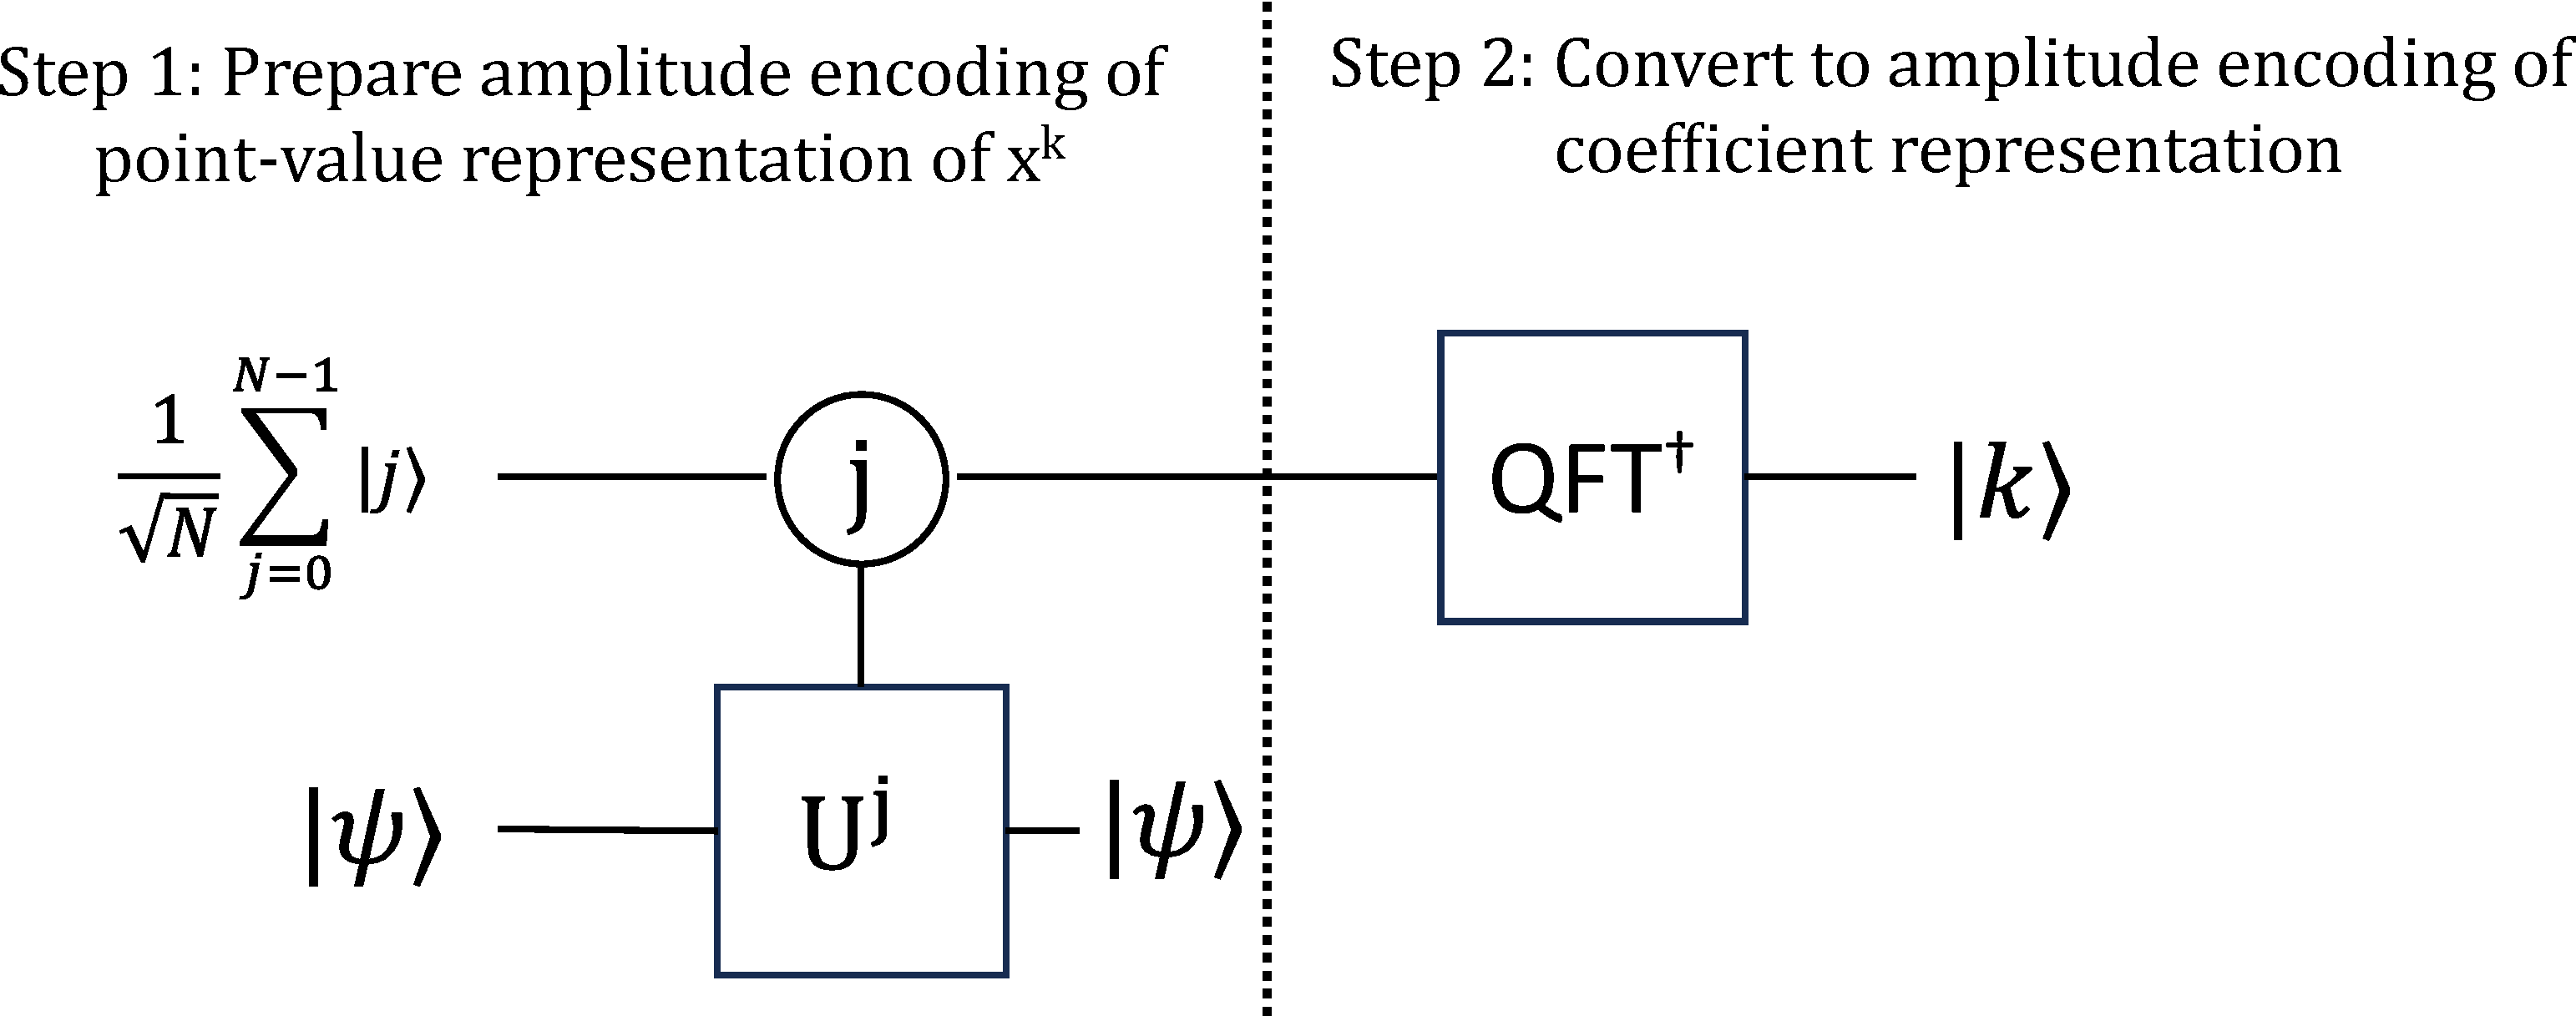
\includegraphics[width=\linewidth]{qpe_circuit.pdf}
		\caption{High level circuit explaining the Quantum Phase Estimation Algorithm. The algorithm has two steps. Step 1 prepares $\frac{1}{\sqrt{N}}\sum_{j=0}^{N-1}  (\omega^{k}_N)^j \ket{j} = \frac{1}{\sqrt{N}}\sum_{j=0}^{N-1}  (\omega^{j}_N)^k \ket{j}$, which is the amplitude encoding of the point-value representation of the polynomial $x^k$. Step 2 converts to the amplitude encoding of the coefficient representation, yielding $k$.}
		\label{fig:qpealgorithm}
	\end{figure}
	
	The Quantum Phase Estimation algorithm is a quantum circuit that uses the qudit-controlled-$U^d$ gate and the quantum state $\ket{\psi}$ to determine the eigenvalue. 
	This circuit has two parts. The first part \textbf{prepares an amplitude encoding of the point-value representation of the polynomial} $\bf{x^k}$. This can be shown from a simple derivation, notice that the resultant state has amplitudes equal to taking each root of unity to the $k$-th power: 
	\begin{eqnarray}
		&C_dU^d [\frac{1}{\sqrt{N}}\sum_{j=0}^{N-1} \ket{j}\ket{\psi}] \nonumber \\
		&=\frac{1}{\sqrt{N}}\sum_{j=0}^{N-1}  (\omega^{k}_N)^j \ket{j} \ket{\psi}  &(\text{Since } U\ket{\psi} = \omega_N^k \ket{\psi}) \nonumber \\
		&=\frac{1}{\sqrt{N}}\sum_{j=0}^{N-1}  (\omega^{j}_N)^k \ket{j} \ket{\psi} 
	\end{eqnarray}
	
	The second part \textbf{converts to the amplitude encoding of the coefficient representation of the polynomial} using the inverse-QFT, giving us the outcome $\ket{k}$ since the polynomial was $x^k$. 
	
	%\section{Quantum Fourier Transform}
	
	%uses the inverse-QFT (which is the inverse-DFT on the amplitudes), 
	%The high-level concepts mentioned in bold in this section are explained in the next subsection. 
	 
	%One last paragraph on how DFT converts 
	
	
	%Polynomials can be stored in classical computers as vectors of coefficients (coefficient representation), or else by simply evaluating the polynomial at a sufficient number of points (point-value representation). In the latter case, we need to evaluate the polynomial at enough points such that the polynomial can be uniquely identified from the points (for example storing two points is enough to uniquely identify a linear function, three points is enough for a quadratic function, etc.). These data structures have different strengths so we want to be able to efficiently convert between them. In particular, choosing to evaluate the polynomial at a set of roots of unity makes this efficient, and this transformation is called the Discrete Fourier Transform. 
	
	%Naive algorithms for this conversion take $O(n^2)$ time, but if the points at which the polynomial is evaluated are chosen to be the roots of unity, then it can be done more efficiently. This transformation is called the Discrete Fourier Transform, and it can be implemented in $O(n \log n)$ time using a divide-and-conquer algorithm called the Fast Fourier Transform algorithm. 
	

	
	
	
	\begin{comment}

	
	\section{Polynomial Data Structures}
	
	This section introduces some background on polynomial data structures, which we will use in our explanation of QPE.
	
	\subsection{The coefficient and point-value representations}
	Polynomials are functions of the form 
	\begin{equation}
	f(x) = a_{n-1} x^{n-1} + ... + a_1 x + a_0.
	\end{equation}
	A natural way to store polynomials in classical computers is thus the \textit{coefficient} representation, i.e. storing $(a_{n-1}, ... ,a_0)$ as a vector. We can choose any sufficiently large $n$ as the size of our vector, which we call the degree-bound (as the degree is \textbf{less} than this number).  Storing polynomials this way gives us familiar algorithms for operating with the polynomials.
	\begin{itemize}
		\item \textbf{Addition:} To add two polynomials, we simply add the two coefficient vectors. This takes $O(n)$ time.
		\item \textbf{Evaluation:} We can evaluate the polynomial on a given input in $O(n)$ time. To do this one has to just avoid computing each power of $x$ independently, as this wastes multiplication operations. One famous trick to achieve this is Horner's rule. 
		\item \textbf{Multiplication:} We can multiply polynomials in $O(n^2)$ time, by means of the familiar long-multiplication algorithm. That is, we would perform the multiplication by the distributive law and collect like-power terms together. As multiplication increases the degree of polynomials, one should check that the resultant polynomial is still degree-bound $n$, but if not, a new vector of appropriate size should be used. 
	\end{itemize}
	   
	The \textit{point-value} representation of polynomials is an alternative data structure that can multiply polynomials in $O(n)$ time. Instead of storing the coefficients, we store the polynomial evaluated at any $n$ inputs of our choosing. For example instead of storing the vector $(1,2,-1,1)$ for $p(x) = x^3 + 2x^2 - x + 1$, we store $(p(0),p(1),p(-1),p(2)) = (1,3,3,15)$.
	
	Once these inputs are chosen, this representation associates a unique vector to each polynomial, because given $n$ points there is a unique degree-bound $n$ polynomial that passes through all those points. For example, given three points on a plane there is either a quadratic function or a line that passes through all three of them. This is because $n$ points give us a system of $n$ linear equations to solve for at most $n$ coefficients of the polynomial. 
	
	In this representation, we can both add and multiply in $O(n)$ time, simply by doing a component-wise addition or multiplication, because $(pq)(x_i) = p(x_i) q(x_i)$. This remains a unique encoding of some polynomial so long as the degree of the resultant polynomial is still less than the degree-bound. 
	
	The trade-off here is that the point-value representation cannot evaluate the polynomial on arbitrary inputs in any straightforward way. 
	
	\subsection{Converting between representations}
	One way to evaluate the polynomial on a given input, we would be able to evaluate the polynomial on arbitrary inputs by converting back to the coefficient representation. 
	
	
	This conversion can be done in $O(n\log n)$ time if we choose a very special set of points, namely the $n$-th roots of unity. 
	
	\section{Quantum Phase Estimation}
	
	Quantum Phase Estimation solves the following computational task:
	\begin{problem*}
		Let $N\in \mathbb{Z}$,$U$ be a unitary, and $\ket{\psi}$ be a quantum state such that $U\ket{\psi} = \omega^k_N \ket{\psi}$ (i.e. $\ket{\psi}$ is an eigenvector of $U$ with eigenvalue that is some $N$-th root of unity.). You are given access to $C_jU^j = \sum_{j=0}^{N-1} \ket{j}\bra{j} \otimes U^j$ gate. Find $k$. 
		\end{problem*}
	
	The Quantum Phase Estimation algorithm has two steps:
	\begin{enumerate}
		\item Prepare the point-value representation of $x^k$, using the $N$-th roots of unity as inputs: 
		
		Perform \begin{align*}
			&C_jU^j [(\frac{1}{\sqrt{N}}\sum_{j=0}^{N-1} \ket{j})\otimes\ket{\psi}] \\
			&=\frac{1}{\sqrt{N}}\sum_{j=0}^{N-1} C_jU^j (\ket{j}\otimes\ket{\psi}) \\
			&=\frac{1}{\sqrt{N}}\sum_{j=0}^{N-1}  (\ket{j}\otimes (\omega^{k}_N)^j\ket{\psi}) \\
			&\underset{\text{(i)}}{=}[\frac{1}{\sqrt{N}}\sum_{j=0}^{N-1}  (\omega^{k}_N)^j \ket{j}]\otimes \ket{\psi} \\
			&\underset{\text{(ii)}}{=}[\frac{1}{\sqrt{N}}\sum_{j=0}^{N-1}  (\omega^{j}_N)^k \ket{j}]\otimes \ket{\psi} \\
		\end{align*}
		The step labelled (i) is simply the moving of constants from one register to the other, and is called ``phase kickback'' as it seems surprising that a phase we think we are applying on $\ket{\psi}$ actually gets applied on the controlling register. In fact, this is only a surprise because of the way we commonly interpret controlled gates, i.e. as being controlled by a controlled register and acting only on the target register. In reality, controlled gates are also two-register interactions and act on the whole system. 
		The step labelled (ii) is the only non-trivial part of our derivation. 
		\item Convert to the coefficient representation to obtain $k$. That is, use the inverse-QFT and measure to obtain $k$. 
		$$ QFT^{\dagger}[\frac{1}{\sqrt{N}}\sum_{j=0}^{N-1}  (\omega^{j}_N)^k \ket{j}] = \ket{k}$$
	\end{enumerate}
	
	
	\end{comment}
	
%	\section{Other motivations}
	
%	John Preskill and Watrous motivate it by starting from the Hadamard test. 
	
%	I perceived the traditional explanations to leave the mechanism of the algorithm up to a computation. It would be left to a "computation by the reader", that the probability of measuring certain outcomes was 0 and hence any outcome is one of the desirable ones. This would mean that circuits were merely stated and could be checked to work by means of computation, but no motivation or explanation was given that might aid in memory or in coming up with new algorithms for oneself. 
	
	
%	A story about QFT and AHSP can be told that sees QFT as mapping from group elements to characters 
	% See https://courses.cs.washington.edu/courses/cse490q/20au/lectures/27-hsp.pdf 

	\bibliographystyle{ieeetr}
	
	\bibliography{References}

	
\end{document}